
% Default to the notebook output style

    


% Inherit from the specified cell style.




    
\documentclass[11pt]{article}

    
    
    \usepackage[T1]{fontenc}
    % Nicer default font (+ math font) than Computer Modern for most use cases
    \usepackage{mathpazo}
	\usepackage{float}
    % Basic figure setup, for now with no caption control since it's done
    % automatically by Pandoc (which extracts ![](path) syntax from Markdown).
    \usepackage{graphicx}
    % We will generate all images so they have a width \maxwidth. This means
    % that they will get their normal width if they fit onto the page, but
    % are scaled down if they would overflow the margins.
    \makeatletter
    \def\maxwidth{\ifdim\Gin@nat@width>\linewidth\linewidth
    \else\Gin@nat@width\fi}
    \makeatother
    \let\Oldincludegraphics\includegraphics
    % Set max figure width to be 80% of text width, for now hardcoded.
    \renewcommand{\includegraphics}[1]{\Oldincludegraphics[width=.8\maxwidth]{#1}}
    % Ensure that by default, figures have no caption (until we provide a
    % proper Figure object with a Caption API and a way to capture that
    % in the conversion process - todo).
    \usepackage{caption}
    \DeclareCaptionLabelFormat{nolabel}{}
    \captionsetup{labelformat=nolabel}

    \usepackage{adjustbox} % Used to constrain images to a maximum size 
    \usepackage{xcolor} % Allow colors to be defined
    \usepackage{enumerate} % Needed for markdown enumerations to work
    \usepackage{geometry} % Used to adjust the document margins
    \usepackage{amsmath} % Equations
    \usepackage{amssymb} % Equations
    \usepackage{textcomp} % defines textquotesingle
    % Hack from http://tex.stackexchange.com/a/47451/13684:
    \AtBeginDocument{%
        \def\PYZsq{\textquotesingle}% Upright quotes in Pygmentized code
    }
    \usepackage{upquote} % Upright quotes for verbatim code
    \usepackage{eurosym} % defines \euro
    \usepackage[mathletters]{ucs} % Extended unicode (utf-8) support
    \usepackage[utf8x]{inputenc} % Allow utf-8 characters in the tex document
    \usepackage{fancyvrb} % verbatim replacement that allows latex
    \usepackage{grffile} % extends the file name processing of package graphics 
                         % to support a larger range 
    % The hyperref package gives us a pdf with properly built
    % internal navigation ('pdf bookmarks' for the table of contents,
    % internal cross-reference links, web links for URLs, etc.)
    \usepackage{hyperref}
    \usepackage{longtable} % longtable support required by pandoc >1.10
    \usepackage{booktabs}  % table support for pandoc > 1.12.2
    \usepackage[inline]{enumitem} % IRkernel/repr support (it uses the enumerate* environment)
    \usepackage[normalem]{ulem} % ulem is needed to support strikethroughs (\sout)
                                % normalem makes italics be italics, not underlines
    \usepackage{mathrsfs}
    

    
    
    % Colors for the hyperref package
    \definecolor{urlcolor}{rgb}{0,.145,.698}
    \definecolor{linkcolor}{rgb}{.71,0.21,0.01}
    \definecolor{citecolor}{rgb}{.12,.54,.11}

    % ANSI colors
    \definecolor{ansi-black}{HTML}{3E424D}
    \definecolor{ansi-black-intense}{HTML}{282C36}
    \definecolor{ansi-red}{HTML}{E75C58}
    \definecolor{ansi-red-intense}{HTML}{B22B31}
    \definecolor{ansi-green}{HTML}{00A250}
    \definecolor{ansi-green-intense}{HTML}{007427}
    \definecolor{ansi-yellow}{HTML}{DDB62B}
    \definecolor{ansi-yellow-intense}{HTML}{B27D12}
    \definecolor{ansi-blue}{HTML}{208FFB}
    \definecolor{ansi-blue-intense}{HTML}{0065CA}
    \definecolor{ansi-magenta}{HTML}{D160C4}
    \definecolor{ansi-magenta-intense}{HTML}{A03196}
    \definecolor{ansi-cyan}{HTML}{60C6C8}
    \definecolor{ansi-cyan-intense}{HTML}{258F8F}
    \definecolor{ansi-white}{HTML}{C5C1B4}
    \definecolor{ansi-white-intense}{HTML}{A1A6B2}
    \definecolor{ansi-default-inverse-fg}{HTML}{FFFFFF}
    \definecolor{ansi-default-inverse-bg}{HTML}{000000}

    % commands and environments needed by pandoc snippets
    % extracted from the output of `pandoc -s`
    \providecommand{\tightlist}{%
      \setlength{\itemsep}{0pt}\setlength{\parskip}{0pt}}
    \DefineVerbatimEnvironment{Highlighting}{Verbatim}{commandchars=\\\{\}}
    % Add ',fontsize=\small' for more characters per line
    \newenvironment{Shaded}{}{}
    \newcommand{\KeywordTok}[1]{\textcolor[rgb]{0.00,0.44,0.13}{\textbf{{#1}}}}
    \newcommand{\DataTypeTok}[1]{\textcolor[rgb]{0.56,0.13,0.00}{{#1}}}
    \newcommand{\DecValTok}[1]{\textcolor[rgb]{0.25,0.63,0.44}{{#1}}}
    \newcommand{\BaseNTok}[1]{\textcolor[rgb]{0.25,0.63,0.44}{{#1}}}
    \newcommand{\FloatTok}[1]{\textcolor[rgb]{0.25,0.63,0.44}{{#1}}}
    \newcommand{\CharTok}[1]{\textcolor[rgb]{0.25,0.44,0.63}{{#1}}}
    \newcommand{\StringTok}[1]{\textcolor[rgb]{0.25,0.44,0.63}{{#1}}}
    \newcommand{\CommentTok}[1]{\textcolor[rgb]{0.38,0.63,0.69}{\textit{{#1}}}}
    \newcommand{\OtherTok}[1]{\textcolor[rgb]{0.00,0.44,0.13}{{#1}}}
    \newcommand{\AlertTok}[1]{\textcolor[rgb]{1.00,0.00,0.00}{\textbf{{#1}}}}
    \newcommand{\FunctionTok}[1]{\textcolor[rgb]{0.02,0.16,0.49}{{#1}}}
    \newcommand{\RegionMarkerTok}[1]{{#1}}
    \newcommand{\ErrorTok}[1]{\textcolor[rgb]{1.00,0.00,0.00}{\textbf{{#1}}}}
    \newcommand{\NormalTok}[1]{{#1}}
    
    % Additional commands for more recent versions of Pandoc
    \newcommand{\ConstantTok}[1]{\textcolor[rgb]{0.53,0.00,0.00}{{#1}}}
    \newcommand{\SpecialCharTok}[1]{\textcolor[rgb]{0.25,0.44,0.63}{{#1}}}
    \newcommand{\VerbatimStringTok}[1]{\textcolor[rgb]{0.25,0.44,0.63}{{#1}}}
    \newcommand{\SpecialStringTok}[1]{\textcolor[rgb]{0.73,0.40,0.53}{{#1}}}
    \newcommand{\ImportTok}[1]{{#1}}
    \newcommand{\DocumentationTok}[1]{\textcolor[rgb]{0.73,0.13,0.13}{\textit{{#1}}}}
    \newcommand{\AnnotationTok}[1]{\textcolor[rgb]{0.38,0.63,0.69}{\textbf{\textit{{#1}}}}}
    \newcommand{\CommentVarTok}[1]{\textcolor[rgb]{0.38,0.63,0.69}{\textbf{\textit{{#1}}}}}
    \newcommand{\VariableTok}[1]{\textcolor[rgb]{0.10,0.09,0.49}{{#1}}}
    \newcommand{\ControlFlowTok}[1]{\textcolor[rgb]{0.00,0.44,0.13}{\textbf{{#1}}}}
    \newcommand{\OperatorTok}[1]{\textcolor[rgb]{0.40,0.40,0.40}{{#1}}}
    \newcommand{\BuiltInTok}[1]{{#1}}
    \newcommand{\ExtensionTok}[1]{{#1}}
    \newcommand{\PreprocessorTok}[1]{\textcolor[rgb]{0.74,0.48,0.00}{{#1}}}
    \newcommand{\AttributeTok}[1]{\textcolor[rgb]{0.49,0.56,0.16}{{#1}}}
    \newcommand{\InformationTok}[1]{\textcolor[rgb]{0.38,0.63,0.69}{\textbf{\textit{{#1}}}}}
    \newcommand{\WarningTok}[1]{\textcolor[rgb]{0.38,0.63,0.69}{\textbf{\textit{{#1}}}}}
    
    
    % Define a nice break command that doesn't care if a line doesn't already
    % exist.
    \def\br{\hspace*{\fill} \\* }
    % Math Jax compatibility definitions
    \def\gt{>}
    \def\lt{<}
    \let\Oldtex\TeX
    \let\Oldlatex\LaTeX
    \renewcommand{\TeX}{\textrm{\Oldtex}}
    \renewcommand{\LaTeX}{\textrm{\Oldlatex}}
    % Document parameters
    % Document title
    \title{Assignment 9}
    \author{Jiarong Ye}
    
    
    
    

    % Pygments definitions
    
\makeatletter
\def\PY@reset{\let\PY@it=\relax \let\PY@bf=\relax%
    \let\PY@ul=\relax \let\PY@tc=\relax%
    \let\PY@bc=\relax \let\PY@ff=\relax}
\def\PY@tok#1{\csname PY@tok@#1\endcsname}
\def\PY@toks#1+{\ifx\relax#1\empty\else%
    \PY@tok{#1}\expandafter\PY@toks\fi}
\def\PY@do#1{\PY@bc{\PY@tc{\PY@ul{%
    \PY@it{\PY@bf{\PY@ff{#1}}}}}}}
\def\PY#1#2{\PY@reset\PY@toks#1+\relax+\PY@do{#2}}

\expandafter\def\csname PY@tok@w\endcsname{\def\PY@tc##1{\textcolor[rgb]{0.73,0.73,0.73}{##1}}}
\expandafter\def\csname PY@tok@c\endcsname{\let\PY@it=\textit\def\PY@tc##1{\textcolor[rgb]{0.25,0.50,0.50}{##1}}}
\expandafter\def\csname PY@tok@cp\endcsname{\def\PY@tc##1{\textcolor[rgb]{0.74,0.48,0.00}{##1}}}
\expandafter\def\csname PY@tok@k\endcsname{\let\PY@bf=\textbf\def\PY@tc##1{\textcolor[rgb]{0.00,0.50,0.00}{##1}}}
\expandafter\def\csname PY@tok@kp\endcsname{\def\PY@tc##1{\textcolor[rgb]{0.00,0.50,0.00}{##1}}}
\expandafter\def\csname PY@tok@kt\endcsname{\def\PY@tc##1{\textcolor[rgb]{0.69,0.00,0.25}{##1}}}
\expandafter\def\csname PY@tok@o\endcsname{\def\PY@tc##1{\textcolor[rgb]{0.40,0.40,0.40}{##1}}}
\expandafter\def\csname PY@tok@ow\endcsname{\let\PY@bf=\textbf\def\PY@tc##1{\textcolor[rgb]{0.67,0.13,1.00}{##1}}}
\expandafter\def\csname PY@tok@nb\endcsname{\def\PY@tc##1{\textcolor[rgb]{0.00,0.50,0.00}{##1}}}
\expandafter\def\csname PY@tok@nf\endcsname{\def\PY@tc##1{\textcolor[rgb]{0.00,0.00,1.00}{##1}}}
\expandafter\def\csname PY@tok@nc\endcsname{\let\PY@bf=\textbf\def\PY@tc##1{\textcolor[rgb]{0.00,0.00,1.00}{##1}}}
\expandafter\def\csname PY@tok@nn\endcsname{\let\PY@bf=\textbf\def\PY@tc##1{\textcolor[rgb]{0.00,0.00,1.00}{##1}}}
\expandafter\def\csname PY@tok@ne\endcsname{\let\PY@bf=\textbf\def\PY@tc##1{\textcolor[rgb]{0.82,0.25,0.23}{##1}}}
\expandafter\def\csname PY@tok@nv\endcsname{\def\PY@tc##1{\textcolor[rgb]{0.10,0.09,0.49}{##1}}}
\expandafter\def\csname PY@tok@no\endcsname{\def\PY@tc##1{\textcolor[rgb]{0.53,0.00,0.00}{##1}}}
\expandafter\def\csname PY@tok@nl\endcsname{\def\PY@tc##1{\textcolor[rgb]{0.63,0.63,0.00}{##1}}}
\expandafter\def\csname PY@tok@ni\endcsname{\let\PY@bf=\textbf\def\PY@tc##1{\textcolor[rgb]{0.60,0.60,0.60}{##1}}}
\expandafter\def\csname PY@tok@na\endcsname{\def\PY@tc##1{\textcolor[rgb]{0.49,0.56,0.16}{##1}}}
\expandafter\def\csname PY@tok@nt\endcsname{\let\PY@bf=\textbf\def\PY@tc##1{\textcolor[rgb]{0.00,0.50,0.00}{##1}}}
\expandafter\def\csname PY@tok@nd\endcsname{\def\PY@tc##1{\textcolor[rgb]{0.67,0.13,1.00}{##1}}}
\expandafter\def\csname PY@tok@s\endcsname{\def\PY@tc##1{\textcolor[rgb]{0.73,0.13,0.13}{##1}}}
\expandafter\def\csname PY@tok@sd\endcsname{\let\PY@it=\textit\def\PY@tc##1{\textcolor[rgb]{0.73,0.13,0.13}{##1}}}
\expandafter\def\csname PY@tok@si\endcsname{\let\PY@bf=\textbf\def\PY@tc##1{\textcolor[rgb]{0.73,0.40,0.53}{##1}}}
\expandafter\def\csname PY@tok@se\endcsname{\let\PY@bf=\textbf\def\PY@tc##1{\textcolor[rgb]{0.73,0.40,0.13}{##1}}}
\expandafter\def\csname PY@tok@sr\endcsname{\def\PY@tc##1{\textcolor[rgb]{0.73,0.40,0.53}{##1}}}
\expandafter\def\csname PY@tok@ss\endcsname{\def\PY@tc##1{\textcolor[rgb]{0.10,0.09,0.49}{##1}}}
\expandafter\def\csname PY@tok@sx\endcsname{\def\PY@tc##1{\textcolor[rgb]{0.00,0.50,0.00}{##1}}}
\expandafter\def\csname PY@tok@m\endcsname{\def\PY@tc##1{\textcolor[rgb]{0.40,0.40,0.40}{##1}}}
\expandafter\def\csname PY@tok@gh\endcsname{\let\PY@bf=\textbf\def\PY@tc##1{\textcolor[rgb]{0.00,0.00,0.50}{##1}}}
\expandafter\def\csname PY@tok@gu\endcsname{\let\PY@bf=\textbf\def\PY@tc##1{\textcolor[rgb]{0.50,0.00,0.50}{##1}}}
\expandafter\def\csname PY@tok@gd\endcsname{\def\PY@tc##1{\textcolor[rgb]{0.63,0.00,0.00}{##1}}}
\expandafter\def\csname PY@tok@gi\endcsname{\def\PY@tc##1{\textcolor[rgb]{0.00,0.63,0.00}{##1}}}
\expandafter\def\csname PY@tok@gr\endcsname{\def\PY@tc##1{\textcolor[rgb]{1.00,0.00,0.00}{##1}}}
\expandafter\def\csname PY@tok@ge\endcsname{\let\PY@it=\textit}
\expandafter\def\csname PY@tok@gs\endcsname{\let\PY@bf=\textbf}
\expandafter\def\csname PY@tok@gp\endcsname{\let\PY@bf=\textbf\def\PY@tc##1{\textcolor[rgb]{0.00,0.00,0.50}{##1}}}
\expandafter\def\csname PY@tok@go\endcsname{\def\PY@tc##1{\textcolor[rgb]{0.53,0.53,0.53}{##1}}}
\expandafter\def\csname PY@tok@gt\endcsname{\def\PY@tc##1{\textcolor[rgb]{0.00,0.27,0.87}{##1}}}
\expandafter\def\csname PY@tok@err\endcsname{\def\PY@bc##1{\setlength{\fboxsep}{0pt}\fcolorbox[rgb]{1.00,0.00,0.00}{1,1,1}{\strut ##1}}}
\expandafter\def\csname PY@tok@kc\endcsname{\let\PY@bf=\textbf\def\PY@tc##1{\textcolor[rgb]{0.00,0.50,0.00}{##1}}}
\expandafter\def\csname PY@tok@kd\endcsname{\let\PY@bf=\textbf\def\PY@tc##1{\textcolor[rgb]{0.00,0.50,0.00}{##1}}}
\expandafter\def\csname PY@tok@kn\endcsname{\let\PY@bf=\textbf\def\PY@tc##1{\textcolor[rgb]{0.00,0.50,0.00}{##1}}}
\expandafter\def\csname PY@tok@kr\endcsname{\let\PY@bf=\textbf\def\PY@tc##1{\textcolor[rgb]{0.00,0.50,0.00}{##1}}}
\expandafter\def\csname PY@tok@bp\endcsname{\def\PY@tc##1{\textcolor[rgb]{0.00,0.50,0.00}{##1}}}
\expandafter\def\csname PY@tok@fm\endcsname{\def\PY@tc##1{\textcolor[rgb]{0.00,0.00,1.00}{##1}}}
\expandafter\def\csname PY@tok@vc\endcsname{\def\PY@tc##1{\textcolor[rgb]{0.10,0.09,0.49}{##1}}}
\expandafter\def\csname PY@tok@vg\endcsname{\def\PY@tc##1{\textcolor[rgb]{0.10,0.09,0.49}{##1}}}
\expandafter\def\csname PY@tok@vi\endcsname{\def\PY@tc##1{\textcolor[rgb]{0.10,0.09,0.49}{##1}}}
\expandafter\def\csname PY@tok@vm\endcsname{\def\PY@tc##1{\textcolor[rgb]{0.10,0.09,0.49}{##1}}}
\expandafter\def\csname PY@tok@sa\endcsname{\def\PY@tc##1{\textcolor[rgb]{0.73,0.13,0.13}{##1}}}
\expandafter\def\csname PY@tok@sb\endcsname{\def\PY@tc##1{\textcolor[rgb]{0.73,0.13,0.13}{##1}}}
\expandafter\def\csname PY@tok@sc\endcsname{\def\PY@tc##1{\textcolor[rgb]{0.73,0.13,0.13}{##1}}}
\expandafter\def\csname PY@tok@dl\endcsname{\def\PY@tc##1{\textcolor[rgb]{0.73,0.13,0.13}{##1}}}
\expandafter\def\csname PY@tok@s2\endcsname{\def\PY@tc##1{\textcolor[rgb]{0.73,0.13,0.13}{##1}}}
\expandafter\def\csname PY@tok@sh\endcsname{\def\PY@tc##1{\textcolor[rgb]{0.73,0.13,0.13}{##1}}}
\expandafter\def\csname PY@tok@s1\endcsname{\def\PY@tc##1{\textcolor[rgb]{0.73,0.13,0.13}{##1}}}
\expandafter\def\csname PY@tok@mb\endcsname{\def\PY@tc##1{\textcolor[rgb]{0.40,0.40,0.40}{##1}}}
\expandafter\def\csname PY@tok@mf\endcsname{\def\PY@tc##1{\textcolor[rgb]{0.40,0.40,0.40}{##1}}}
\expandafter\def\csname PY@tok@mh\endcsname{\def\PY@tc##1{\textcolor[rgb]{0.40,0.40,0.40}{##1}}}
\expandafter\def\csname PY@tok@mi\endcsname{\def\PY@tc##1{\textcolor[rgb]{0.40,0.40,0.40}{##1}}}
\expandafter\def\csname PY@tok@il\endcsname{\def\PY@tc##1{\textcolor[rgb]{0.40,0.40,0.40}{##1}}}
\expandafter\def\csname PY@tok@mo\endcsname{\def\PY@tc##1{\textcolor[rgb]{0.40,0.40,0.40}{##1}}}
\expandafter\def\csname PY@tok@ch\endcsname{\let\PY@it=\textit\def\PY@tc##1{\textcolor[rgb]{0.25,0.50,0.50}{##1}}}
\expandafter\def\csname PY@tok@cm\endcsname{\let\PY@it=\textit\def\PY@tc##1{\textcolor[rgb]{0.25,0.50,0.50}{##1}}}
\expandafter\def\csname PY@tok@cpf\endcsname{\let\PY@it=\textit\def\PY@tc##1{\textcolor[rgb]{0.25,0.50,0.50}{##1}}}
\expandafter\def\csname PY@tok@c1\endcsname{\let\PY@it=\textit\def\PY@tc##1{\textcolor[rgb]{0.25,0.50,0.50}{##1}}}
\expandafter\def\csname PY@tok@cs\endcsname{\let\PY@it=\textit\def\PY@tc##1{\textcolor[rgb]{0.25,0.50,0.50}{##1}}}

\def\PYZbs{\char`\\}
\def\PYZus{\char`\_}
\def\PYZob{\char`\{}
\def\PYZcb{\char`\}}
\def\PYZca{\char`\^}
\def\PYZam{\char`\&}
\def\PYZlt{\char`\<}
\def\PYZgt{\char`\>}
\def\PYZsh{\char`\#}
\def\PYZpc{\char`\%}
\def\PYZdl{\char`\$}
\def\PYZhy{\char`\-}
\def\PYZsq{\char`\'}
\def\PYZdq{\char`\"}
\def\PYZti{\char`\~}
% for compatibility with earlier versions
\def\PYZat{@}
\def\PYZlb{[}
\def\PYZrb{]}
\makeatother


    % Exact colors from NB
    \definecolor{incolor}{rgb}{0.0, 0.0, 0.5}
    \definecolor{outcolor}{rgb}{0.545, 0.0, 0.0}



    
    % Prevent overflowing lines due to hard-to-break entities
    \sloppy 
    % Setup hyperref package
    \hypersetup{
      breaklinks=true,  % so long urls are correctly broken across lines
      colorlinks=true,
      urlcolor=urlcolor,
      linkcolor=linkcolor,
      citecolor=citecolor,
      }
    % Slightly bigger margins than the latex defaults
    
    \geometry{verbose,tmargin=1in,bmargin=1in,lmargin=1in,rmargin=1in}
    
    

    \begin{document}
    
    
    \maketitle
    
    

    
    \textbf{1.Brainstorming}.

A researcher investigated whether brainstorming is more effective for
larger groups than for smaller ones by setting up four groups of
agribusiness executives, the group sizes being two, three, four, and
five, respectively. He also set up four groups of agribusiness
scientists, the group sizes being the same as for the agribusiness
executives. The researcher gave each group the same problem: ``How can
Canada increase the value of its agricultural exports?'' Each group was
allowed 30 minutes to generate ideas. The variable of interest was the
number of different ideas proposed by the group. The results, classified
by type of group (factor A) and size of group (factor B), were:

\begin{figure}[H]
\centering
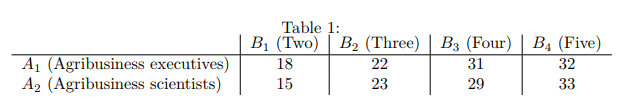
\includegraphics{1.png}
\caption{}
\end{figure}

\textbf{Assume that no-interaction ANOVA model is appropriate.}

    \subsubsection*{Q1}\label{q1}

\begin{enumerate}
\def\labelenumi{\arabic{enumi}.}
\tightlist
\item
  20 points Plot the data in an interaction plot. Does it appear that
  interaction effects are present? Does it appear that factor A and
  factor B main effects are present? Discuss
\end{enumerate}

    \begin{Verbatim}[commandchars=\\\{\}]
{\color{incolor}In [{\color{incolor}6}]:} A \PY{o}{=} \PY{k+kt}{c}\PY{p}{(}\PY{k+kp}{rep}\PY{p}{(}\PY{l+s}{\PYZdq{}}\PY{l+s}{A1\PYZdq{}}\PY{p}{,} \PY{l+m}{4}\PY{p}{)}\PY{p}{,} \PY{k+kp}{rep}\PY{p}{(}\PY{l+s}{\PYZdq{}}\PY{l+s}{A2\PYZdq{}}\PY{p}{,} \PY{l+m}{4}\PY{p}{)}\PY{p}{)}
        B \PY{o}{=} \PY{k+kp}{rep}\PY{p}{(}\PY{k+kt}{c}\PY{p}{(}\PY{l+s}{\PYZsq{}}\PY{l+s}{B1\PYZsq{}}\PY{p}{,} \PY{l+s}{\PYZsq{}}\PY{l+s}{B2\PYZsq{}}\PY{p}{,} \PY{l+s}{\PYZsq{}}\PY{l+s}{B3\PYZsq{}}\PY{p}{,} \PY{l+s}{\PYZsq{}}\PY{l+s}{B4\PYZsq{}}\PY{p}{)}\PY{p}{,} \PY{l+m}{2}\PY{p}{)}
        num\PYZus{}ideas \PY{o}{=} \PY{k+kt}{c}\PY{p}{(}\PY{l+m}{18}\PY{p}{,} \PY{l+m}{22}\PY{p}{,} \PY{l+m}{31}\PY{p}{,} \PY{l+m}{32}\PY{p}{,} \PY{l+m}{15}\PY{p}{,} \PY{l+m}{23}\PY{p}{,} \PY{l+m}{29}\PY{p}{,} \PY{l+m}{33}\PY{p}{)}
        df \PY{o}{=} \PY{k+kt}{data.frame}\PY{p}{(}A \PY{o}{=} A\PY{p}{,} B\PY{o}{=}B\PY{p}{,} num\PYZus{}ideas\PY{o}{=}num\PYZus{}ideas\PY{p}{)}
        df
\end{Verbatim}

    \begin{tabular}{r|lll}
 A & B & num\_ideas\\
\hline
	 A1 & B1 & 18\\
	 A1 & B2 & 22\\
	 A1 & B3 & 31\\
	 A1 & B4 & 32\\
	 A2 & B1 & 15\\
	 A2 & B2 & 23\\
	 A2 & B3 & 29\\
	 A2 & B4 & 33\\
\end{tabular}


    
    \begin{Verbatim}[commandchars=\\\{\}]
{\color{incolor}In [{\color{incolor}11}]:} interaction.plot\PY{p}{(}x.factor \PY{o}{=} df\PY{o}{\PYZdl{}}B\PY{p}{,} trace.factor \PY{o}{=} df\PY{o}{\PYZdl{}}A\PY{p}{,}
                             response \PY{o}{=} df\PY{o}{\PYZdl{}}num\PYZus{}ideas\PY{p}{,} type \PY{o}{=}\PY{l+s}{\PYZdq{}}\PY{l+s}{b\PYZdq{}}\PY{p}{,}col \PY{o}{=} \PY{l+m}{2}\PY{o}{:}\PY{l+m}{3}\PY{p}{,}
                             xlab \PY{o}{=}\PY{l+s}{\PYZdq{}}\PY{l+s}{group size\PYZdq{}}\PY{p}{,} ylab \PY{o}{=}\PY{l+s}{\PYZdq{}}\PY{l+s}{Number of ideas\PYZdq{}}\PY{p}{,}
                             trace.label \PY{o}{=}\PY{l+s}{\PYZdq{}}\PY{l+s}{concentration\PYZdq{}}\PY{p}{)}
\end{Verbatim}

    \begin{center}
    \adjustimage{max size={0.9\linewidth}{0.9\paperheight}}{output_3_0.png}
    \end{center}
    { \hspace*{\fill} \\}
    
    The interaction plot shows a weak interaction, with the lines for
concentration=A1 and concentration=A2 being nearly parallel.

Factor A main effects are not present because with with factor A on the
Y axis, the the lines for concentration A1 and A2 are almost overlapping
each other, indicating that for each one of factor B, there's no
significant difference between A1 and A2.

Factor B main effects are present because with factor B on the X axis,
the lines for concentration A1 and A2 are not horizontal, the absolute
value of slope is relatively large, indicating that for each one of
factor A, there's significant difference among B1 to B4, thus we could
conclude that factor A is present.

    \subsubsection*{Q2}\label{q2}

\begin{enumerate}
\def\labelenumi{\arabic{enumi}.}
\setcounter{enumi}{1}
\tightlist
\item
  40 points (By hand) Conduct separate tests for type of group and size
  of group main effects. In each test, use level of significance α =
  0.01 and state the alternatives, decision rule, and conclusion. What
  is the P-value for each test?
\end{enumerate}

    \[\mu_{..} = \frac{18+15+22+23+31+29+32+33}{8} = 25.375\]

\[\mu_{A1.} = \frac{18+22+31+32}{4} = 25.75\]

\[\mu_{A2.} = \frac{15+23+29+33}{4} = 25\]

\[\mu_{B1.} = \frac{18+15}{2} = 16.5\]

\[\mu_{B2.} = \frac{22+23}{2} = 22.5\]

\[\mu_{B3.} = \frac{31+29}{2} = 30\]

\[\mu_{B4.} = \frac{32+33}{2} = 32.5\]

\[SS_A = 4 \cdot (25.75-25.375)^2 + 4 \cdot (25 - 25.375)^2 = 1.125\]

\[SS_B = 2 \cdot (16.5 - 25.375)^2 + 2 \cdot (22.5 - 25.375)^2 + 2 \cdot (30 - 25.375)^2 + 2 \cdot (32.5 - 25.375)^2 = 318.375\]

\[MS_A = \frac{SS_A}{Df} = 1.125\]

\[MS_B = \frac{SS_B}{Df} = \frac{318.375}{3} = 106.125\]

\[SS_{total} = (18 - 25.375)^2 + (22 - 25.375)^2 + (31 - 25.375)^2 + (32 - 25.375)^2 + (15 - 25.375)^2\]

\[+ (23 - 25.375)^2+ (29 - 25.375)^2+ (33 - 25.375)^2 = 325.875\]

\[SSE = SS_{total} - SS_A - SS_B = 325.875 - 1.125 - 106.125 = 6.375\]

\[MSE = \frac{SSE}{Df} = \frac{6.375}{3} = 2.125\]

\[F_A = \frac{MS_A}{MSE} = \frac{1.125}{2.125} = 0.529\]

\[F_B = \frac{MS_B}{MSE} = \frac{106.125}{2.125} = 49.941\]

Two-way ANOVA table :


\begin{figure}[H]
	\centering
	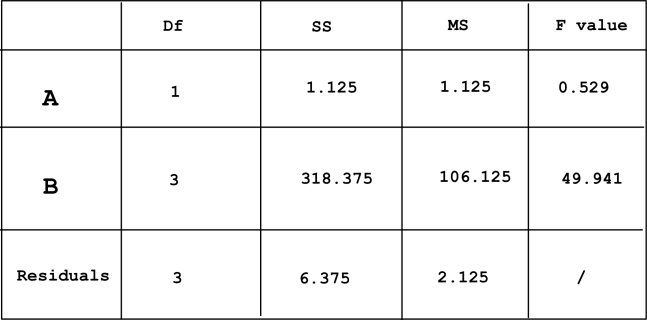
\includegraphics{2.png}
	\caption{}
\end{figure}


    \begin{Verbatim}[commandchars=\\\{\}]
{\color{incolor}In [{\color{incolor}12}]:} \PY{c+c1}{\PYZsh{} check my answer:}
         modelAB\PY{o}{\PYZlt{}\PYZhy{}}aov\PY{p}{(}num\PYZus{}ideas\PY{o}{\PYZti{}}A\PY{o}{+}B\PY{p}{,} data\PY{o}{=}df\PY{p}{)}
         anova\PY{p}{(}modelAB\PY{p}{)}
\end{Verbatim}

\[\]

    \begin{tabular}{r|lllll}
  & Df & Sum Sq & Mean Sq & F value & Pr(>F)\\
\hline
	A & 1           &   1.125     &   1.125     &  0.5294118  & 0.519497962\\
	B & 3           & 318.375     & 106.125     & 49.9411765  & 0.004641637\\
	Residuals & 3           &   6.375     &   2.125     &         NA  &          NA\\
\end{tabular}

\[\]

    
    \textbf{For factor A (type of group):}

Null hypothesis:

\[H_0: \alpha_1 = \alpha_2 = 0\]


Alternative:

\[H_1: \text{ there exists at least one in } \alpha_1, \alpha_2 \text{ that's not } 0\]

since the p value \(p = 0.519 > 0.01\), so we are not confident enough
to reject the null hypothesis, thus we could make the conclusion that
there are no significant difference between factor $\alpha_1$ and $\alpha_2$.
It is consistent with the result we got from the interaction plot above
that the factor A main effects are not present.

\textbf{For factor B (size of group):}

Null hypothesis:

\[H_0: \beta_1 = \beta_2 = \beta_3 = \beta_4 = 0\]

Alternative:
\[H_1: \text{ there exists at least one in } \beta_1, \beta_2, \beta_3, \beta_4 \text{ that's not } 0\]

since the p value \(p = 0.0046 < 0.01\), so we are confident enough to
reject the null hypothesis, thus we could make the conclusion that there
are significant difference among factor \(\beta_1\) to \(\beta_4\). It is
consistent with the result we got from the interaction plot above that
the factor B main effects are present.

    \subsubsection*{Q3}\label{q3}

\begin{enumerate}
\def\labelenumi{\arabic{enumi}.}
\setcounter{enumi}{2}
\tightlist
\item
  40 points (By hand) Obtain confidence intervals for
  \(D_1 = \mu_{·2} − \mu_{·1} ,D_2 = \mu_{·3} − \mu_{·2}, D_3 = \mu_{·4} - \mu_{·3}\);
  use the Bonferroni procedure with a 95 percent family confidence
  coefficient. State your findings.
\end{enumerate}

    \begin{Verbatim}[commandchars=\\\{\}]
{\color{incolor}In [{\color{incolor}42}]:} \PY{k+kn}{library}\PY{p}{(}multcomp\PY{p}{)}
         \PY{k+kp}{summary}\PY{p}{(}glht\PY{p}{(}aov\PY{p}{(}num\PYZus{}ideas\PY{o}{\PYZti{}}A\PY{o}{+}B\PY{p}{,} data \PY{o}{=} df\PY{p}{)}\PY{p}{,} linfct \PY{o}{=} mcp\PY{p}{(}B \PY{o}{=} \PY{l+s}{\PYZsq{}}\PY{l+s}{Tukey\PYZsq{}}\PY{p}{)}\PY{p}{)}\PY{p}{)}
\end{Verbatim}

    
    \begin{verbatim}

	 Simultaneous Tests for General Linear Hypotheses

Multiple Comparisons of Means: Tukey Contrasts


Fit: aov(formula = num_ideas ~ A + B, data = df)

Linear Hypotheses:
             Estimate Std. Error t value Pr(>|t|)   
B2 - B1 == 0    6.000      1.458   4.116  0.07553 . 
B3 - B1 == 0   13.500      1.458   9.261  0.00802 **
B4 - B1 == 0   16.000      1.458  10.976  0.00494 **
B3 - B2 == 0    7.500      1.458   5.145  0.04217 * 
B4 - B2 == 0   10.000      1.458   6.860  0.01905 * 
B4 - B3 == 0    2.500      1.458   1.715  0.44723   
---
Signif. codes:  0 ‘***’ 0.001 ‘**’ 0.01 ‘*’ 0.05 ‘.’ 0.1 ‘ ’ 1
(Adjusted p values reported -- single-step method)

    \end{verbatim}

    
    \[\hat D_1 = \mu_{2} - \mu_{1} = \frac{22+23}{2} - \frac{18+15}{2} = 6\]

\[\hat D_2 = \mu_{·3} − \mu_{·2} = \frac{31+29}{2} - \frac{22+23}{2} = 7.5\]

\[\hat D_3 = \mu_{·4} - \mu_{·3} = \frac{32+33}{2} - \frac{31+29}{2} = 2.5\]

\[S(\hat D_1) = S(\hat D_2) = S(\hat D_3) = \sqrt{MSE \cdot (\frac{1}{2} + \frac{1}{2})} = 1.458\]

\[B = t(1 - \alpha/(2g); \: df_A \cdot df_B) = t(1 - 0.05/6; 3) = t(0.99167; 3)\]

    \begin{Verbatim}[commandchars=\\\{\}]
{\color{incolor}In [{\color{incolor}45}]:} qt\PY{p}{(}\PY{l+m}{0.99167}\PY{p}{,} \PY{l+m}{3}\PY{p}{)}
\end{Verbatim}

    4.8573697522534

    
    \[\therefore B = 4.857\]

Thus, using the Bonferroni procedure, the 95\% family-wise CI for
\(D_1 , D_2\) and \(D_3\) is:

\[D_1: 6 \pm 4.857 \cdot 1.458 = [-1.08, 13.08]\]

\[D_2: 7.5 \pm 4.857 \cdot 1.458 = [0.42, 14.58]\]

\[D_3: 2.5 \pm 4.857 \cdot 1.458 = [-4.58, 9.58]\]

From the CI above, since 0 is included in the CI of \(D_1, D_3\), 0 not
included in the CI of \(D_2\), thus we can conclude that there's
significant difference between \(\mu_{3}\) and \(\mu_{2}\), with
\(\mu_{3}\) significantly larger than \(\mu_{2}\); there not enough
confidence to guarantee that there exists significant difference between
\(\mu_{2}\) and \(\mu_{1}\), \(\mu_{4}\) and \(\mu_{3}\).

  

    % Add a bibliography block to the postdoc
    
    
    
    \end{document}
